\chapter{Evaluation Harnesses, Contamination, and Statistical Validity}\label{ch:C26}
AgentHorizon and TestJack provide October 2026 examples of why evaluation logic belongs inside the scientific object being compared~\cite{corpus261011050,yao2026testjack}. A trajectory-aware computer-use judge and a coding witness-test auditor observe different evidence and target different mistakes. Their results should therefore alter the design of a comparison before they alter a leaderboard: define which property the instrument observes, audit its errors, and retain the configured execution that produced the artifact.

An evaluation harness is an experimental instrument. It constructs observations, constrains actions, allocates resources, records outcomes, and applies a scoring rule. Errors in any of those functions can change a measured capability claim. A benchmark name and a model name are therefore insufficient to identify an experiment. The evaluated object is the configured model-policy-harness-environment system under a particular sampling and scoring protocol.

This chapter develops the estimands, controls, implementation checks, and uncertainty analysis needed to interpret agent results. The aim is not to replace all benchmarks with one universal score. It is to make comparisons answer a precise question and to expose when apparently conflicting results concern different populations, information budgets, or evaluator behavior.

\section{Define the estimand before the leaderboard}\label{sec:C26:estimand}
Let $D$ be a task distribution, $S$ a system configuration, $B$ a resource envelope, and $Y$ a declared outcome. The primary estimand can be written $\mu(S,B,D)=\mathbb E_{x\sim D}[Y(S,B,x)]$. Formally, $D$ is a probability measure on an eligible task space $\mathcal X$, and $Y$ is integrable under the joint task and execution randomness; a normalized success outcome has range $[0,1]$. Every symbol carries a substantive choice. Tasks can be sampled by repository, user, domain, or time. Resources can constrain money, elapsed time, attempts, or tool access. Outcomes can measure final correctness, constraints, latency, or utility. A numerical ranking is uninterpretable without these choices.

Micro- and macro-averages answer different questions. A micro-average weights each task equally, so a large task family dominates. A macro-average gives equal weight to families, potentially giving a small noisy group disproportionate influence. Neither is universally correct. Report the weighting rule and family-level results, and avoid changing weights after seeing which system benefits. Where a deployment distribution is known, a workload-weighted estimate can be relevant, but its sampling uncertainty and drift remain material.

The system boundary should include model checkpoint or service identity, prompt and harness revision, tools, memory policy, evaluator, and environment. A benchmark score obtained with a newer parser or different hidden-test version is a different observation even if the headline labels are unchanged. Closed service revisions may be unavailable; then the result is a dated service evaluation rather than a fully reproducible checkpoint comparison.

The foundational 2022 HELM framework emphasizes multidimensional evaluation across scenarios and metrics~\cite{liang2022helm}. For agents, this perspective extends naturally to permission compliance, state consistency, external effects, and recovery. A system can improve success while worsening cost or security. A scalar utility can summarize those tradeoffs only after the weights and acceptable constraints are justified. It should not conceal a hard safety or authorization requirement inside a favorable average.

The practical first step is an evaluation contract that names the target population, eligibility rules, unit of analysis, allowed information, resource limits, stopping conditions, and outcome definitions. This contract supports later auditing because it makes deviations visible. It also prevents an experiment from drifting into a different question when difficult cases or infrastructure failures appear.


% SCIENTIFIC_FIGURE_C26
Figure~\ref{fig:C26:overview} contrasts selection feedback with the one-way transfer of a frozen artifact to sealed evaluation.
\begin{figure}[!htbp]
\centering
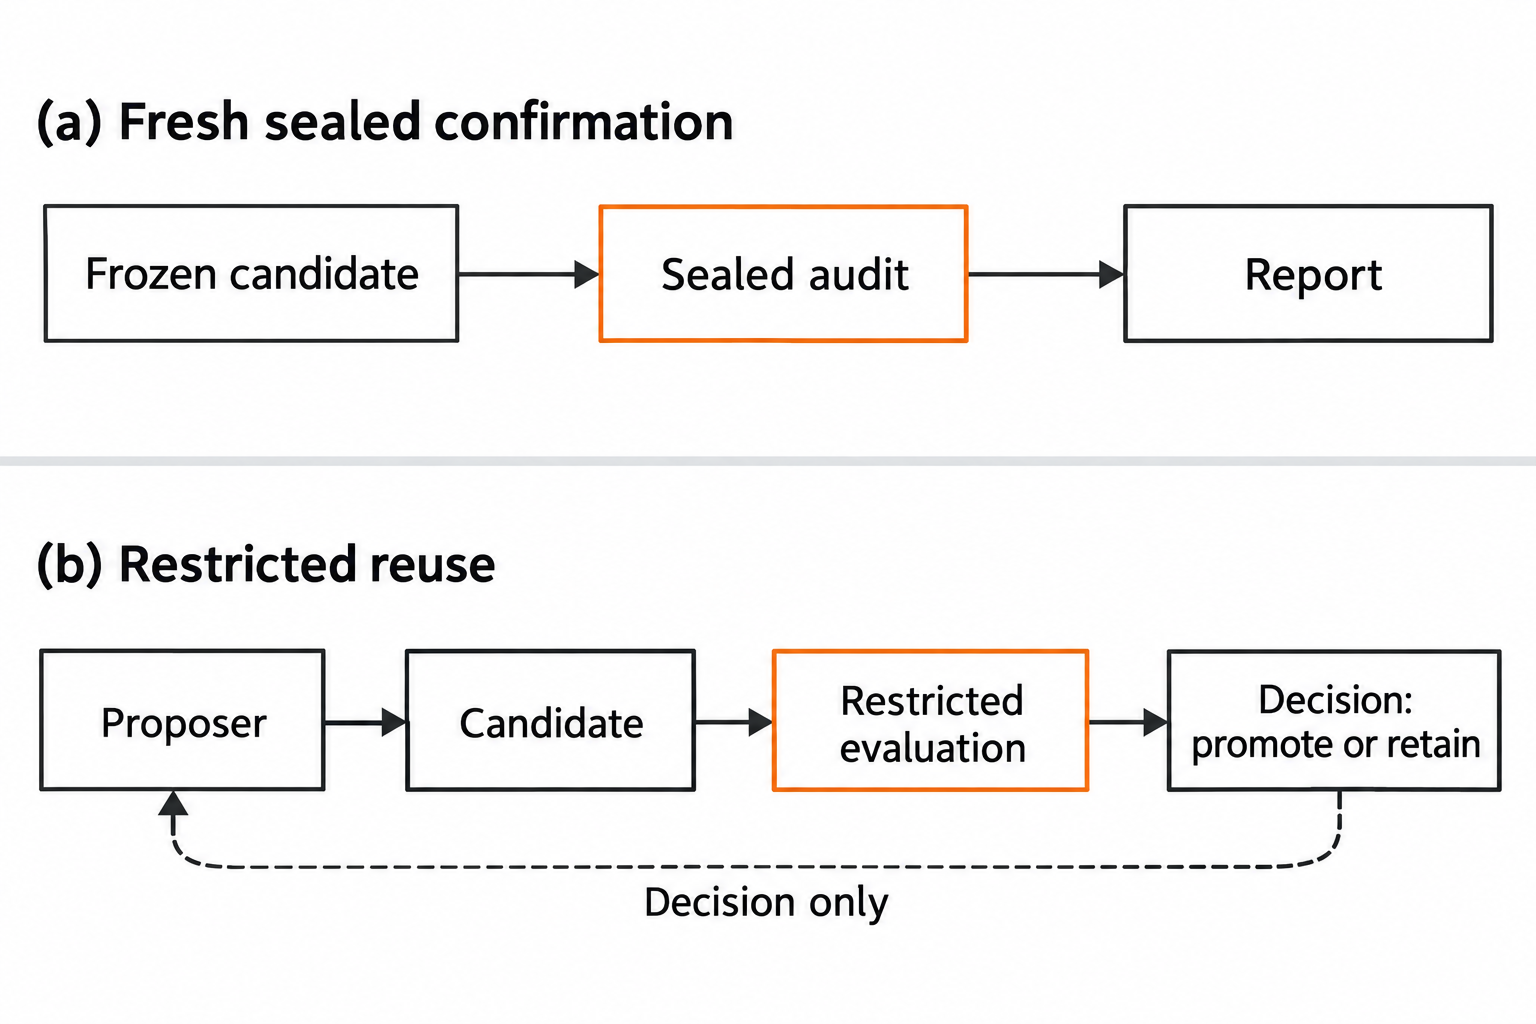
\includegraphics[width=\linewidth]{book/figures/assets/F26review.png}
\caption{Two evaluation protocols with distinct feedback boundaries. Fresh sealed confirmation returns a report outside selection. Restricted reuse exposes only promotion decisions to the proposer; validity additionally requires the source protocol's initial evaluation independence and history-wide error allocation. The feedback restriction alone is not an error-control proof. No experimental outcomes are depicted.}
\label{fig:C26:overview}
\end{figure}

\section{Harness construction and artifact identity}\label{sec:C26:construction}
The harness controls initial state and evaluator access. For repository tasks, it selects the checkout, installs dependencies, exposes the issue description, and later runs tests. For browser tasks, it resets application databases and authentication state. For memory tasks, it decides what persists across episodes. Each reset policy can leak information or remove difficulty if implemented incorrectly.

The inspected language-model evaluation harness exposes evaluation entry points, while SWE-bench's harness exposes instance execution and aggregation paths~\cite{repo_lm_eval,jimenez2023swebench}. These are concrete implementation anchors, not evidence that every downstream adapter is valid. An audit should follow one task through construction, action execution, result serialization, and score aggregation. Check that the scorer reads the artifact generated by that task rather than an old file, cached response, or another worker's output.

Stable identifiers should connect task, attempt, environment, artifact, and verdict. A directory name alone is weak identity when workers reuse workspaces. Content digests and immutable manifests reduce ambiguity. The manifest should include test selection and evaluator configuration because a result can change when the same artifact is judged under a different rule. A successful container exit code does not establish that the intended tests ran.

Environment failures require explicit classification. Dependency installation can fail, a website can change, a tool can become unavailable, or the evaluator can crash. These failures affect operational reliability even when they do not diagnose model reasoning. Report both overall task success and conditional policy performance under valid infrastructure, with clear denominators. Removing failed setup cases after observing outcomes can bias comparisons if one system stresses infrastructure differently.

Sandbox isolation protects benchmark validity as well as deployment security. Hidden tests, reference artifacts, and scores must not be readable by the agent unless the protocol intentionally provides them. Shared caches and logs can create indirect leakage. A deterministic fixture should attempt to read forbidden paths and query evaluator state to verify the boundary. Such checks establish concrete isolation properties rather than relying on the phrase sandboxed environment.


\section{Attempts reliability and selection}\label{sec:C26:attempts}
Finding one successful answer among several attempts differs from succeeding reliably on repeated execution. Under independent identical success probability $p$, the former is $1-(1-p)^k$ and the latter is $p^k$. These formulas are illustrative models, not general laws for agent systems. Attempts can share task difficulty, memory, environment state, or sampling behavior, making their joint distribution substantially different.

For $n$ sampled candidates with $c$ successes, the familiar combinatorial pass-at-$k$ estimator is $1-\binom{n-c}{k}/\binom{n}{k}$ when the sampling and interpretation conditions apply~\cite{chen2021codeeval}. The domain is $1\leq k\leq n$ and $0\leq c\leq n$, all integers, with $\binom{n-c}{k}=0$ when $k>n-c$. It estimates discovery of a success among selected candidates, not a deployable selector's performance. An actual system needs a gate that identifies a valid candidate without access to hidden labels. Selector false acceptance and false rejection belong inside end-to-end evaluation.

For a fixed realized candidate set, that expression is exactly the fraction of uniformly chosen size-$k$ subsets containing a success. Its interpretation as an unbiased estimate of fresh $k$-attempt discovery additionally needs the corresponding exchangeable sampling model; adaptive revisions are not automatically such samples. Task heterogeneity introduces a separate distinction. If attempts are independent conditional on task $q$ with success probability $p(q)$, then
\begin{equation}
 \theta_{\mathrm{any},k}=\mathbb E_q[1-(1-p(q))^k],\qquad
 \theta_{\mathrm{all},k}=\mathbb E_q[p(q)^k].
\end{equation}
For integer $k\geq1$ and $\bar p=\mathbb E_q[p(q)]$, Jensen's inequality gives $\theta_{\mathrm{any},k}\leq1-(1-\bar p)^k$ and $\theta_{\mathrm{all},k}\geq\bar p^k$. Thus even conditional independence does not justify raising a pooled mean to a power. These are analytical comparisons under the stated model, not estimates of any cited benchmark's reliability.

Attempt budgets should count failed parsing, tool errors, and abandoned generations where they consume resources. The mini-swe-agent accounting change discussed in Chapter~\ref{ch:C23} illustrates why this is implementation-sensitive. Equal nominal attempts can hide unequal token use or paid failed calls. Report measured cost and consumed resources rather than only configured maxima.

Repeated-run reliability should retain the benchmark's exact definition. Some protocols ask whether every repetition succeeds; others measure average success or consistency of a required constraint. A paper using one definition cannot be compared directly with another merely because both use a superscript or similar label. State the aggregation rule in ordinary language and provide the underlying per-task outcomes when possible.

Adaptive selection increases the effective search budget. A system that repeatedly revises prompts, harnesses, or memory using benchmark feedback has used the benchmark as an optimization resource. RRSI explicitly addresses overfitting in harness evolution~\cite{rrsi2026}. The evaluation should preserve an untouched assessment set and record candidate counts, rejected changes, and evaluator access. Frozen weights do not imply absence of learning from test feedback.

An untouched confirmation set is one design; certified reuse requires a different protocol. REUSE permits feedback-adaptive proposals only through promotion decisions from an initially independent evaluation sample and allocates error across all possible promotion histories~\cite{ch02_reuse2026}. Returning detailed scores or failure traces to the proposer breaks that theorem's decision-only restriction unless the extra transcript is accounted for. A generic confidence sequence protects optional stopping under its assumptions; it does not erase information already leaked into candidate construction. The public report should therefore describe the feedback channel as precisely as the tested artifact.


\section{Contamination information leakage and task lineage}\label{sec:C26:contamination}
Contamination is not a single binary property. A model may have seen the exact task, a near duplicate, the reference patch, a discussion of the solution, or a related repository version. A harness may leak hidden tests at runtime. Persistent memory can transfer answer-bearing information from previous evaluation episodes. Each channel requires a different control and supports a different inference about generalization.

Use task lineage to track duplicates and revisions. A later benchmark release can contain transformed versions of earlier public tasks. Deduplication based only on exact text can miss equivalent code changes or renamed entities. Semantic similarity is useful for screening but can also flag legitimately related tasks. Report the screening procedure and unresolved cases rather than claim complete decontamination from one similarity threshold.

Temporal holdouts reduce some exposure but do not guarantee novelty. A task first published after model training may depend on a public issue or patch that predates the cutoff. Conversely, a benchmark revision date does not make an old task new. Record first public availability of the task and solution separately when evidence permits. For proprietary models, unknown training data limits what can be established.

Runtime leakage should be tested directly. Keep evaluator credentials outside the agent environment, separate reference artifacts, and inspect tool access. A browser agent can inadvertently observe a success marker or database field intended only for grading. A coding agent can discover test files copied into the wrong layer. These are implementation defects that can be fixed without speculative claims about model memorization.

Memory experiments require explicit contamination boundaries. If one arm carries experiences across tasks while another resets, the information difference is the treatment and must be reported. If a learned skill contains a benchmark-specific answer rather than a reusable procedure, transfer gains can reflect memorization. Holdouts should test both new instances and changed task structure, with source and experience provenance available for audit.

\subsection{Interference through persistent state}\label{sec:C26:stateinterference}
A stateful benchmark generally does not admit independent per-task potential outcomes. Let $X_{1:t}$ be the task prefix, $M_t^S$ the memory generated by system $S$ on that prefix, and $Y_t(S,M_t^S,X_t)$ the next outcome. Changing the system at an early task changes later memory and therefore later outcomes even when the task list is fixed. A mean over tasks estimates performance of the complete stream policy under its order and feedback rules; it does not identify an isolated memory effect at every task.

Two experiments answer different questions. A frozen-prefix experiment initializes both arms from the same admissible state and varies the next decision mechanism. A full-stream experiment initializes a common starting state and lets each arm construct its own subsequent memory. The former isolates a conditional local effect; the latter measures accumulated adaptation and error propagation. Resetting memory after every task removes the longitudinal treatment, while copying the stronger arm's evolved bank into both conditions changes the treatment again. Report the chosen intervention and cluster uncertainty by independently generated stream. Chapter~\ref{ch:C27} develops the corresponding counterfactual controls and contamination boundaries.

\section{Uncertainty paired designs and dependence}\label{sec:C26:uncertainty}
An agent evaluation has several sources of variation: task sampling, model sampling, environment nondeterminism, evaluator error, and adaptive state. Treating every model call as an independent observation ignores most of this structure. The appropriate uncertainty analysis follows the unit to which the claim generalizes. Repository-level generalization needs variation across repositories, not merely many attempts on the same few issues.

Paired comparisons reduce nuisance variation by evaluating systems on the same task instances. Define $\Delta_i=Y_{i,A}-Y_{i,B}$ and estimate its mean over the target population. Confidence intervals should preserve pairing. If tasks cluster by user, repository, or persistent session, resample clusters or use an explicitly justified hierarchical model. The choice should be declared before inspecting which interval is narrower.

Repeated seeds estimate stochastic execution variation conditional on the sampled tasks. They do not substitute for broader task coverage. Conversely, one run on many tasks can estimate a task-population average while leaving repeated-run reliability uncertain. Report both dimensions when the deployment depends on consistency. If compute prevents sufficient replication, narrow the claim rather than inventing stability from a positive mean.

Multiplicity matters when researchers compare many models, prompts, memory mechanisms, and metrics. Selecting the best configuration and reporting an ordinary confidence interval as if it had been fixed in advance understates uncertainty. Separate exploration from confirmation, report the selection procedure, and use untouched data for final comparison. A universal correction is not required for every descriptive analysis, but the inferential claim must reflect how the configuration was chosen.

Missing and censored outcomes need visible treatment. A timeout may indicate excessive latency, infrastructure failure, or an unfinished but promising trajectory. For a deadline-constrained task it is a failure to meet the deadline, regardless of possible eventual success. Additional analyses can examine completion-time distributions, but they should not erase the primary operational outcome. Report sensitivity to reasonable classification choices when the cause is ambiguous.


\section{Ablations and causal mechanism claims}\label{sec:C26:ablations}
An ablation removes or changes a mechanism, but it can also change resources, information, and optimization opportunities. Removing a retrieval module may shorten the context and reduce cost; removing a critic may reduce model calls; replacing a hypergraph with flat retrieval may alter both representation and access policy. The observed difference identifies the combined treatment unless additional controls isolate the components.

HyperSkill provides a useful example. Its no-hypergraph condition replaces the structured retrieval pipeline with flat embedding retrieval, so the result does not isolate hyperedge representation alone~\cite{xu2026hyperskill}. A stronger comparison keeps decomposition, candidate pools, ranking budget, and maintenance cost comparable while varying the storage relation. This does not invalidate the system result; it narrows the causal explanation supported by that ablation.

Oracle controls estimate headroom. Oracle retrieval tests whether downstream reasoning can use sufficient evidence; oracle state tests whether partial observation is the bottleneck; an oracle selector tests candidate-generation potential. These controls are deliberately privileged. Their performance cannot be described as deployable capability, but the gaps help prioritize engineering work. A large oracle-retrieval gap suggests retrieval deserves attention before increasing reasoning depth.

Negative controls test whether a supposed mechanism is doing meaningful work. Shuffle memory, provide irrelevant skills, randomize delegation messages, or replace a feature description with a plausible wrong label. Some controls can damage the system in several ways, so interpret them carefully. The aim is not to produce a dramatic drop but to distinguish a specific explanation from alternatives such as extra context, extra compute, or evaluator bias.

A mechanism claim requires explicit operating conditions and failure regimes. It identifies where the mechanism helps, where a simpler baseline matches it, and where it causes regressions. This is more useful than a universal superiority claim because deployments occupy particular workloads. Method comparisons should therefore preserve heterogeneity across horizon, task structure, evidence quality, and tool reliability rather than compress everything into one average.


\section{Evaluator audits and reproducible reporting}\label{sec:C26:audit}
Evaluators need their own validation set and error analysis. A benchmark can be well constructed while a particular grader accepts artifacts that violate requirements. AgentHorizon and TestJack expose different aspects of this problem: long-trajectory judgment and insufficient executable tests~\cite{corpus261011050,yao2026testjack}. The appropriate response is to audit the observation and scoring pipeline, not merely add another model judge and call the result verified.

October 2026 harness evaluations expose additional estimand boundaries. TraceTrial-Bench preserves raw operational states but resolves some unexercised criteria using the task outcome, so its semantic harness and task scores are coupled; its selected execution archive does not supply independent repetitions within every cell~\cite{ch01_tracetrial2026}. ASAP's frozen-base-model measurements include reference-prefix elicitation and bounded recovery, whereas Harness Scaling evaluates training exposure and transfer to withheld execution combinations~\cite{ch01_asap2026,ch01_harnessscaling2026}. An audit must retain those interventions in its configuration ledger. Treating all three as ordinary backbone leaderboards would discard the variable each study is designed to examine.

Preserve raw verdicts, reason codes, evidence links, and subsequent adjudications. If an evaluator is corrected, publish both original and revised outcomes with the rule change. A moving grader can otherwise make historical comparisons impossible. Where legal or privacy constraints prevent releasing trajectories, provide a precise description of what remains inaccessible and what external investigators can still reproduce.

The reporting record should contain task manifest, environment construction, model and harness identities, prompts, tool schemas, memory policy, budgets, seed policy, evaluator revision, and complete outcomes. Logs should distinguish no response from empty response, unknown usage from zero usage, and incomplete work from completed failure. These distinctions affect both cost and capability estimates.

Reproducibility is graded rather than binary. Metadata verification establishes identity. Source inspection establishes an implementation path. Executed fixtures establish behavior under controlled conditions. Independent replication tests whether reported results recur. Cross-environment reproduction tests robustness to implementation and infrastructure differences. A survey should name the achieved level for each source rather than allow a verified title to imply verified experimental evidence.

The practical endpoint is a comparison whose conclusion can be reconstructed from its records. Another investigator should be able to identify what changed, which observations supported the score, how uncertainty was computed, and which failures remain unresolved. That standard does not require pretending that every proprietary component is transparent. It requires making opacity an explicit limit on inference rather than filling it with plausible assumptions.

\section{A concrete audit of a paired repository comparison}\label{sec:C26:pairedcase}
Consider two coding systems evaluated on the same repository-task manifest. The manifest names the base commit, issue description, dependency environment, required tests, and allowed resource envelope. Each system produces one primary attempt and optional additional attempts under a separately declared budget. The experiment's primary question is deadline-constrained verified completion, not whether a successful patch can eventually be found with unlimited retries. Defining this question before execution determines how timeouts and infrastructure problems enter the analysis.

The harness first constructs an isolated environment and records its identity. The system receives the task and permitted tools, but not the reference patch or hidden evaluator. At termination, the harness freezes the produced artifact, records its digest, and runs the evaluator against that digest. If the artifact changes during evaluation, the run is invalid and must be diagnosed rather than scored against a moving target. This sequence is directly auditable in the task construction, execution and scoring code paths.

The inspected SWE-bench execution module exposes \path{run_instance} and \path{run_instances}; the language-model evaluation harness exposes \path{simple_evaluate} and \texttt{evaluate}. These names identify concrete entry points for examining how tasks become outcomes\cite{jimenez2023swebench,repo_lm_eval}. Their presence does not establish that a custom adapter passes the intended arguments or that an experiment used the inspected revision. The ledger must connect the callable to actual configuration and recorded execution before calling the result reproduced.

Table~\ref{tab:C26:ledger} specifies the evidence needed at each boundary. The table contains no measured outcome. It is a testable contract for distinguishing model errors from deterministic evaluation defects.
\begingroup\setlength{\tabcolsep}{3pt}\small
\begin{longtable}{L{24mm}L{41mm}L{43mm}}
\caption{Evidence boundaries in a repository evaluation.}\label{tab:C26:ledger}\\
\toprule Boundary & Required identity or observation & Failure to expose \\
\midrule\endfirsthead
\toprule Boundary & Required identity or observation & Failure to expose \\
\midrule\endhead
Task construction & Task ID, base commit, dependency manifest, reset policy. & A reused checkout contains a previous answer or a changed dependency. \\
Model context & Prompt digest, tool schemas, accessible history and memory scope. & One arm receives additional solution-bearing context. \\
Execution & Attempt ID, tool calls, costs, timeouts and environment events. & Failed paid calls disappear from the budget record. \\
Artifact freeze & Patch or commit digest and creation time. & Tests run on a different artifact from the submitted one. \\
Grading & Evaluator revision, selected tests, raw verdict and error status. & Evaluator failure is interpreted as an ordinary negative result or omitted. \\
Aggregation & Eligibility denominator, pairing and missing-outcome policy. & Difficult failed runs are excluded after their outcomes are known. \\
Confirmation & Untouched tasks and fixed final configuration. & Repeated holdout tuning is reported as independent assessment. \\
\bottomrule\end{longtable}
\endgroup

Suppose some outcomes remain unresolved because the evaluator failed after execution. A success rate computed only over resolved runs is a conditional quantity. Without assumptions about missingness, it cannot identify the overall task success rate. If there are $N$ eligible runs, $s$ confirmed successes and $u$ unresolved outcomes, a simple identification interval is $[s/N,(s+u)/N]$ when all other outcomes are confirmed failures. The interval expresses missing information; it is not a confidence interval for task sampling.

This distinction matters when systems fail differently. One system may generate patches that stress the evaluator and cause more unresolved runs. Excluding them can make it appear better even if they are concentrated among difficult cases. Conversely, scoring every evaluator crash as a model failure mixes infrastructure and policy behavior. Report the overall operational outcome and a cause-stratified analysis, while retaining a sensitivity analysis for unresolved cases. Do not choose the classification after seeing which ordering it favors.

For paired comparison, preserve the outcome pair for each task. Tasks where both systems succeed contribute differently from tasks where only one succeeds. A test based on discordant pairs can be useful under its assumptions, but repository clustering or persistent memory can violate independence between pairs. A cluster-aware bootstrap or hierarchical analysis should then follow the declared task-generation structure. More attempts on the same repository do not create independent evidence about new repositories.

Resource matching requires another audit. If system A retries malformed outputs while system B stops, equal configured call limits can conceal different paid usage. Record actual model and tool consumption. If one arm receives more wall-clock because its environment starts faster, decide whether startup is part of the deployment comparison or a nuisance variable to control. Both choices can be legitimate; silently switching between them cannot. A complete report shows configured ceilings and realized consumption.

The evaluator should also inspect null and reference conditions. The unmodified repository reveals whether the benchmark's tests already pass without a fix. The reference patch reveals whether the intended environment can represent the benchmark's declared solution. A null pass can indicate inadequate tests; a reference failure can indicate environment drift or benchmark defects. Neither result should be attributed to the evaluated agent. These controls establish whether the instrument can distinguish the states it is intended to score.

Finally, add an independent audit of accepted patches. Dynamic witness tests can expose behavior missing from the fixed suite, while requirement review prevents incidental reference choices from becoming new obligations. Keep the original and audited scores separate, identify the sampled passing-trial population, and cluster uncertainty by task. A revised acceptance criterion changes the estimand; documenting that change makes the evidence more useful rather than less impressive. The result is a comparison whose limitations are concrete enough to guide the next experiment.

An additional distinction concerns cost per successful task. Dividing total cost by confirmed successes can be operationally informative, but it is unstable when success is rare and can hide differences in task mix. Report total eligible tasks, confirmed successes, unresolved outcomes and aggregate cost alongside the ratio. If a system fails quickly on hard tasks, it may have low average cost per attempt without being efficient at useful work. If it spends heavily to rescue difficult cases, its average attempt cost can rise while its cost per accepted deliverable improves. The relevant conclusion depends on which work the deployment must complete, not on whichever denominator yields the smaller number.

The benchmark should preserve outcome severity as well as success. A task that returns no patch, a patch that fails tests, and a patch that passes tests while changing access controls all count differently in an operational loss model. The primary benchmark can retain a binary completion definition for comparability, but a secondary failure taxonomy should record those distinctions. Severity weights require domain justification and sensitivity analysis. They should not be tuned to favor the preferred system after the failures are known. This analysis is particularly important when moving from isolated coding containers to tools that can affect external users.

Releasing the comparison also requires attention to provenance and confidentiality. A trace can contain credentials, private code, personal data or hidden evaluator material. Redaction should preserve event identity, timing, error categories and the evidence needed to reconstruct the score while removing content that cannot be shared. If redaction removes decisive evidence, state the resulting reproduction limit explicitly. A public summary and a private complete audit are different evidence products. Neither should be represented as the other. The scientific requirement is an honest account of which claims an independent reader can actually check from the released artifacts.

A signed manifest can bind the released task list, artifact digests and scoring configuration, reducing ambiguity about which experimental objects a later reproduction attempts to reconstruct.

